\documentclass[a4paper, 10pt]{article}
\usepackage[utf8]{inputenc}
\usepackage{verbatim}
\usepackage{listings}
\usepackage{graphicx}
\usepackage{a4wide}
\usepackage{color}
\usepackage{amsmath}
\usepackage{amssymb}
\usepackage[dvips]{epsfig}
\usepackage[toc,page]{appendix}
\usepackage[T1]{fontenc}
\usepackage{cite} % [2,3,4] --> [2--4]
\usepackage{shadow}
\usepackage{hyperref}
\usepackage{titling}
\usepackage{marvosym }
\usepackage{subcaption}
\usepackage[noabbrev]{cleveref}
\usepackage{wasysym}


\renewcommand{\topfraction}{.85}
\renewcommand{\bottomfraction}{.7}
\renewcommand{\textfraction}{.15}
\renewcommand{\floatpagefraction}{.66}
\renewcommand{\dbltopfraction}{.66}
\renewcommand{\dblfloatpagefraction}{.66}
\setcounter{topnumber}{9}
\setcounter{bottomnumber}{9}
\setcounter{totalnumber}{20}
\setcounter{dbltopnumber}{9}


\setlength{\droptitle}{-10em}   % This is your set screw

\setcounter{tocdepth}{2}

\lstset{language=c++}
\lstset{alsolanguage=[90]Fortran}
\lstset{basicstyle=\small}
\lstset{backgroundcolor=\color{white}}
\lstset{frame=single}
\lstset{stringstyle=\ttfamily}
\lstset{keywordstyle=\color{red}\bfseries}
\lstset{commentstyle=\itshape\color{blue}}
\lstset{showspaces=false}
\lstset{showstringspaces=false}
\lstset{showtabs=false}
\lstset{breaklines}
\date{}
\title{FYS2150 - Prelab2}
\author{Gunnar Lange\\ Username:gunnalan}
\begin{document}

\maketitle
\begin{enumerate}
\item \textbf{A}
\item \textbf{B}
\item \textbf{C}
\item \textbf{E}
\item \textbf{B}
\item \textbf{C}
\item \textbf{A}
\item \textbf{A}
\item \textbf{C}
\item \textbf{B}, avtar
\item \textbf{D}
\end{enumerate}

Plottene er vist nedenfor:
\begin{figure}[!ht]
    \centering
    \begin{subfigure}[H!]{0.5\textwidth}
        \centering
        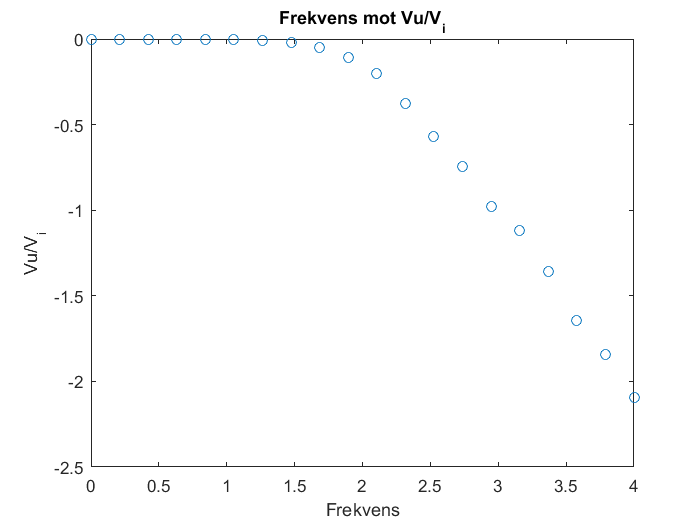
\includegraphics[height=2.4in]{FmotVu.png}
        \caption{Plott av datasett}
            \end{subfigure}%
    ~ 
    \begin{subfigure}[H!]{0.5\textwidth}
        \centering
        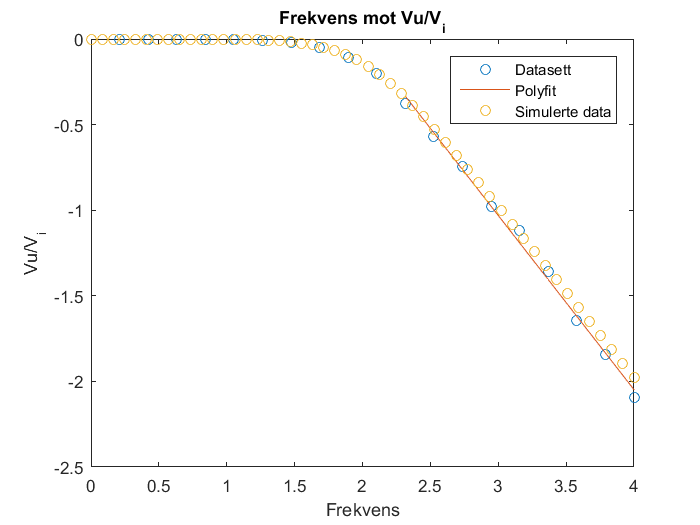
\includegraphics[height=2.4in]{FmotVu_og_simulert.png}
        \caption{Plott av datasett, polyfit og simulerte data}
    \end{subfigure}
\end{figure}


\end{document}